\chapter{Methodology}
\label{sec:methodology}
The methodology applied to optimize the HDC model for an FPGA implementation consists of four parts. First, two implementation-level improvements reduce redundant computation without changing the HDC model itself. Second, the hypervectors stored in the CCIM are optimized using a genetic algorithm with the goal of maintaining or improving classification accuracy at lower vector dimensions $D$. Third, different quantization techniques are investigated to reduce the number of quantization levels $L$ and therefore the size of the CCIM. Finally, the resulting HDC model is implemented as a pipelined and parallelized SystemC accelerator and synthesized to \ac{RTL} for FPGA implementation. 

\section{Implementation-Level Improvements}
\label{sec:implementation_improvements}
Before optimizing the HDC representation itself, two implementation improvements are applied that reduce computational effort without changing the underlying HDC model. 
\enlargethispage{\baselineskip}
The first improvement is an N-gram buffer. Since N-grams are constructed from overlapping sequences, each spatially encoded sample occurs in up to $N$ consecutive N-grams. With the baseline value $N = 3$, a sample first appears in the last position of an N-gram, then in the middle position of the following N-gram, and finally in the first position of the third N-gram. A naive implementation that spatially encodes all three samples whenever an N-gram is constructed consequently encodes each sample up to three times. To avoid this redundant computation, a FIFO buffer stores the most recent spatially encoded hypervectors. The spatial encoder inserts each encoded sample into the buffer only once, and once the buffer contains $N$ samples, the temporal encoder constructs a new N-gram whenever a new sample is added. The oldest sample is then discarded from the buffer. For sufficiently long sequences, this reduces the number of spatial encoding operations by approximately a factor of $N=3$. \\

The second improvement concerns a hardware-oriented implementation of bundling. As described in Equation \ref{eq:binary-bundling}, binary bundling is based on an element-wise majority vote. A direct implementation accumulates the number of ones at each vector position and compares the result with a threshold corresponding to half the number of bundled vectors. Instead, the accumulation can be reformulated by adding +1 for every vector element equal to 1 and -1 for every element equal to 0. The resulting signed accumulator directly determines the output bit. A non-negative value results in a one, while a negative value results in a zero. This formulation is mathematically equivalent to the direct implementation of bundling but replaces the explicit threshold at half the number of bundled hypervectors with a comparison against zero. It is therefore used as the bundling operation in the hardware-oriented SystemC implementation.


\section{Genetic Optimization of CCIM Representation}
\label{sec:GA}

As discussed in Section \ref{sec:optimizationOfHDCRelatedWork}, Basaklar et al. show that the distances between consecutive level hypervectors can be optimized using a \ac{GA} to improve the HDC representation, particularly at reduced vector dimensions \cite{basaklar_hypervector_2021}. The method developed in this work is based on this approach and adapted to the baseline HDC model for EMG classification.

As the optimization target, for each feature $f$, a bit-flip vector $\mathbf{b}^f = [b^f_0,b^f_1,\ldots,b^f_{L-2}]$ of length $L-1$ is defined. The $i$-th element $b_i^f$ contains the number of bits that are flipped to obtain the level hypervector $\boldsymbol{\ell}^f_{i+1}$ from $\boldsymbol{\ell}^f_i$. Consequently, $b^f_i$ directly corresponds to the Hamming distance between these two consecutive level hypervectors. The indices of the bits to be flipped are selected according to a feature-specific random permutation, as described in Section \ref{sec:baseline_item_memory}. 
The bit-flip vectors $\mathbf{b}^f$ of all $F$ features are combined into the optimization matrix $\mathbf{B}$

\[
\mathbf{B}
=
\begin{bmatrix}
\mathbf{b}^0\\
\mathbf{b}^1\\
\vdots\\
\mathbf{b}^{F-1}
\end{bmatrix}
\in \mathbb{N}_0^{F\times(L-1)}.
\]
Thus, one individual in the GA is represented by one complete matrix $\mathbf{B}$, while one row $\mathbf{b}^f$ determines the CIM geometry of a single EMG feature.

For every feature, the total number of bit flips, and therefore the sum over all elements of $\mathbf{b}^f$, is constrained to the number of hypervector dimensions $D$ as defined in Equation \ref{eq:sum_constraint}. 

\begin{equation}
\sum_{i=0}^{L-2} b_i^f = D
\label{eq:sum_constraint}
\end{equation}

In the following, this requirement is referred to as the sum constraint. Since the feature-specific permutation contains every hypervector-dimension index exactly once, every vector dimension is consequently flipped exactly once between the first and last level hypervectors $\boldsymbol{\ell}^f_{0}$ and $\boldsymbol{\ell}^f_{L-1}$, making these two binary hypervectors complements. For a conventional equally spaced CIM, this flip budget is distributed uniformly across the $L-1$ transitions, resulting in $b^f_i \approx D/(L-1)$.

Figure \ref{fig:cim_generation_comparison} illustrates the effect on the CIM of changing $\mathbf{b}^f$ as performed by the \ac{GA}. The example uses $D=12$ and $L=4$. The equally spaced CIM on the left distributes the flip budget equally with $\mathbf{b}^f=[4,4,4]$, while the non-equally spaced example on the right uses $\mathbf{b}^f=[2,7,3]$. For readability, the first level hypervector $\boldsymbol{\ell}^f_{0}$ is chosen as the zero vector and the permutation follows the natural order of the vector indices. In the actual implementation, both the initial hypervector and the permutation are generated randomly.

\begin{figure}[htbp]
    \centering

    \begin{minipage}[t]{0.48\textwidth}
        \centering
        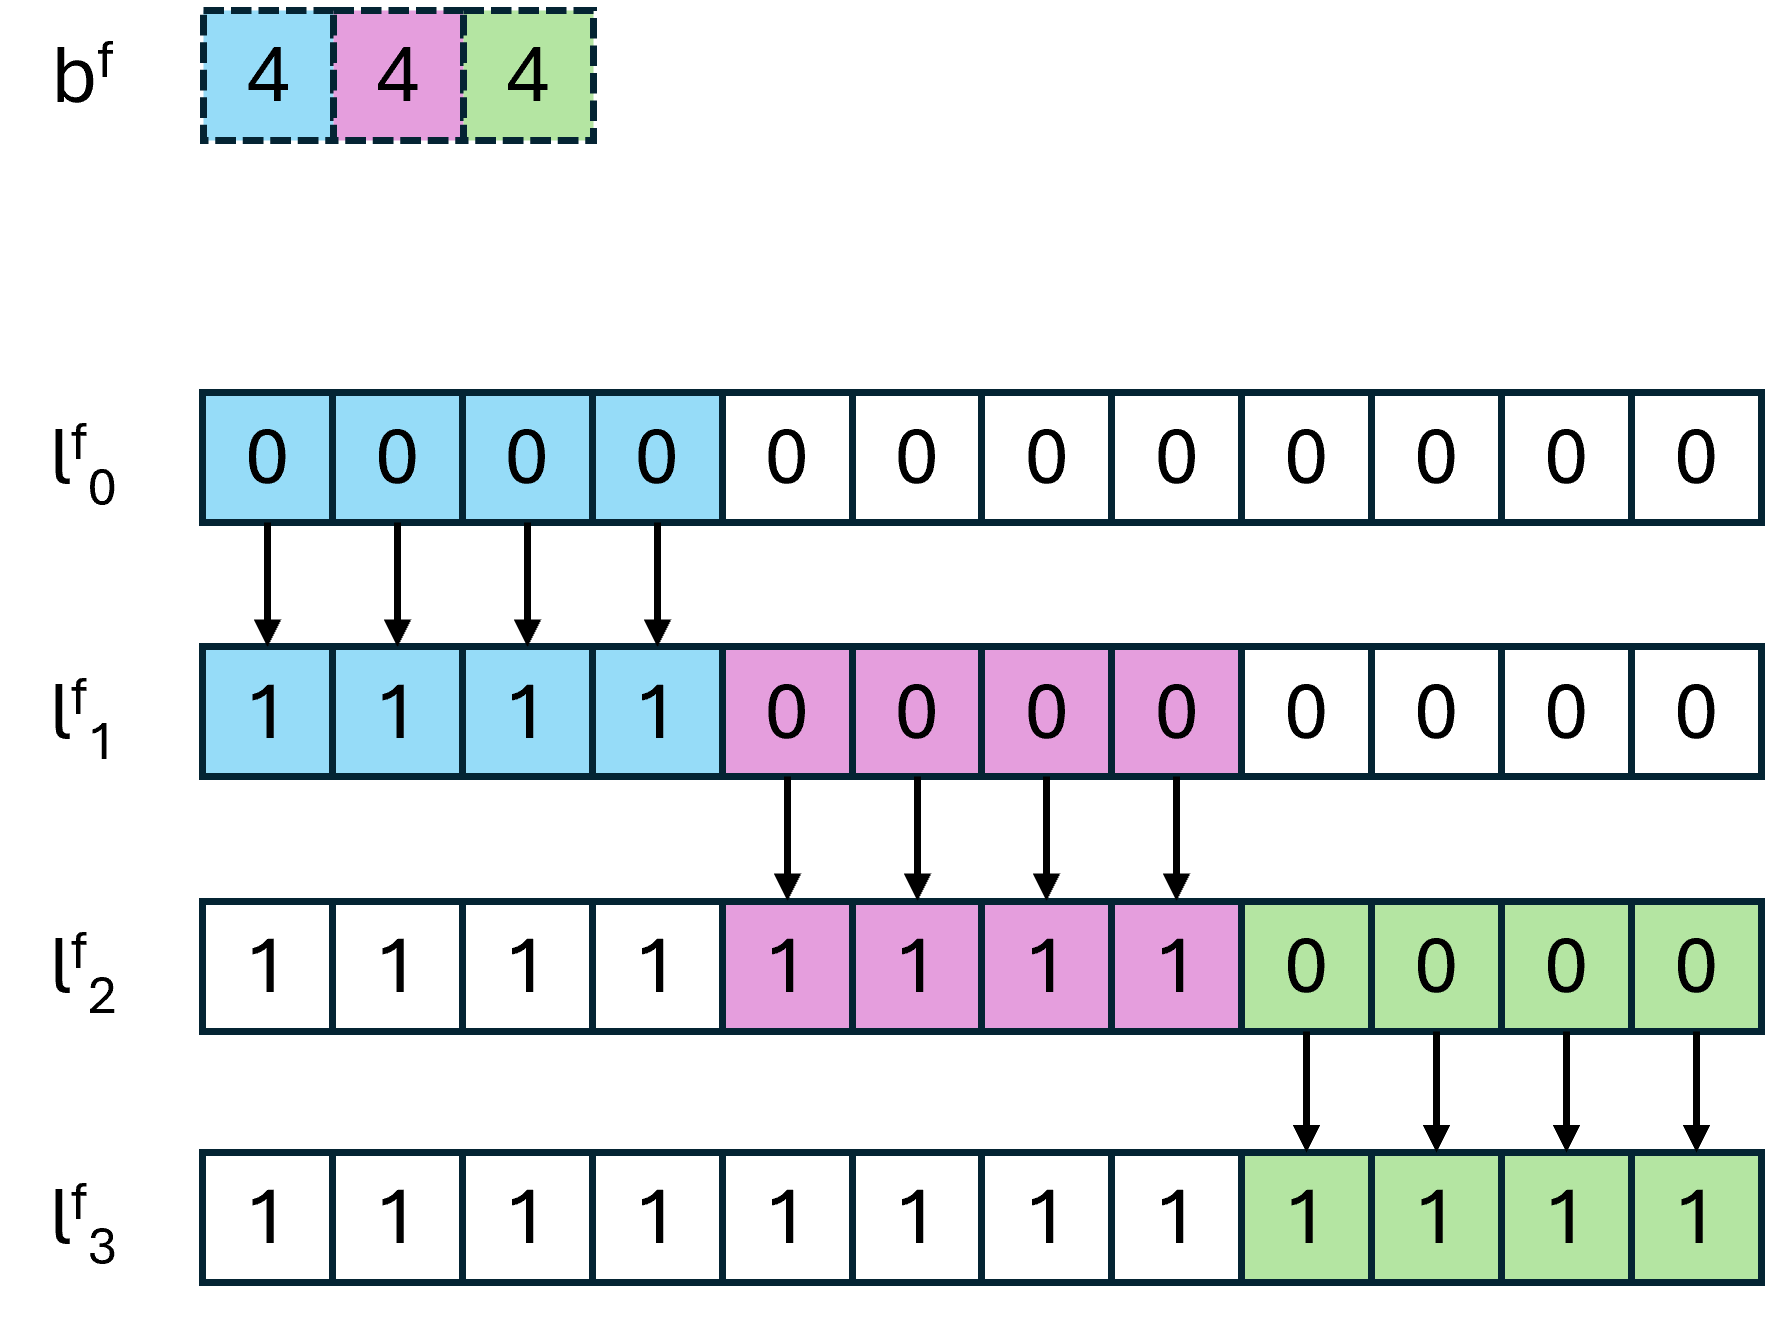
\includegraphics[width=\linewidth]{Images/bToCimNaive.png}

        \vspace{0.3em}
        \textbf{(a) Equally distributed bit-flip vector and corresponding CIM}
        \label{fig:cim_equal_spaced}
    \end{minipage}
    \hfill
    \begin{minipage}[t]{0.48\textwidth}
        \centering
        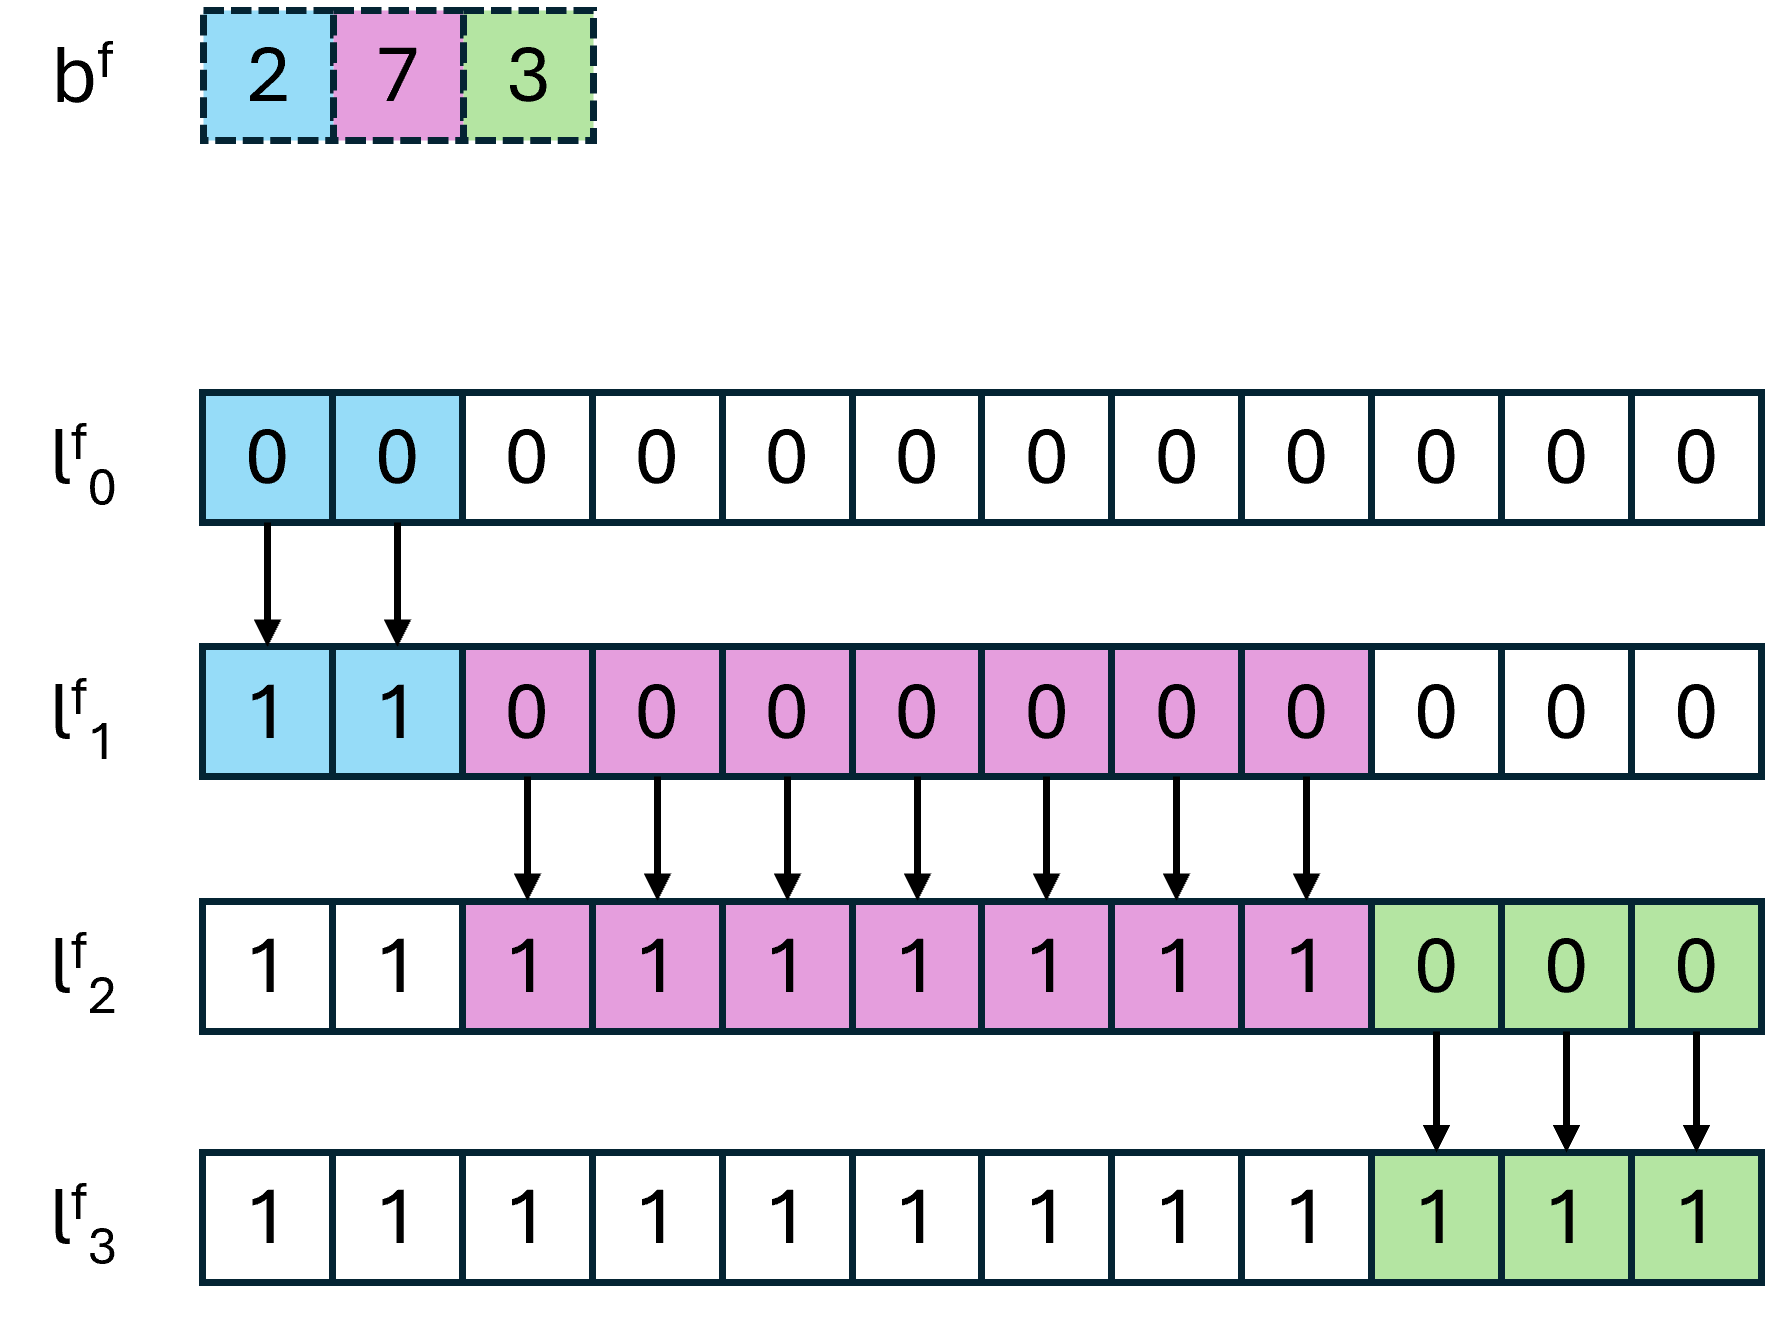
\includegraphics[width=\linewidth]{Images/bToCimOptimized.png}

        \vspace{0.3em}
        \textbf{(b) Non-equally distributed bit-flip vector and corresponding CIM}
        \label{fig:cim_distributed}
    \end{minipage}

    \caption{Illustrative comparison of equally spaced and non-equally distributed CIM generation for one feature. In both examples, the vector dimension is $D=12$ and the number of level transitions is three.}
    \label{fig:cim_generation_comparison}
\end{figure}

In the equally spaced example, every pair of consecutive level hypervectors has a Hamming distance of four. For the non-equally spaced example on the right with $\mathbf{b}^f=[2,7,3]$, the distance between level hypervectors $\boldsymbol{\ell}^f_{1}$ and $\boldsymbol{\ell}^f_{2}$ is increased to seven, while fewer bit flips are assigned to the other transitions. If distinguishing values mapped to levels 1 and 2 is particularly relevant for classification, this larger distance provides stronger separation between their representations in the hyperdimensional space $\mathcal{H}$. The central idea is therefore to redistribute the available bit-flip budget across the level transitions according to their relevance for the classification task, with the aim of increasing class vector separation and improving classification accuracy and robustness.\\

Which transitions should receive larger or smaller distances depends on the feature and the underlying EMG data and cannot be determined directly. Therefore, the complete bit-flip matrix $\mathbf{B}$ is optimized using a \ac{GA}. The optimization procedure is summarized in Algorithm \ref{alg:ga_cim_optimization}.

Initially, a population of $P$ bit-flip matrices $\mathbf{B}$ is generated. Although the equally spaced baseline matrix would provide an obvious starting point, initializing the complete population around this representation would reduce the diversity of the initial search space and could lead to premature convergence. Instead, a diverse initial population is generated by randomly distributing the fixed flip budget $D$ over the $L-1$ level transitions independently for every feature. For each row $\mathbf{b}^f$, random weights are drawn for all transitions, normalized to the total flip budget $D$, and rounded to integer values. A final correction ensures compliance with the sum constraint. For all GA experiments in this work, the population size is set to $P=128$, the number of generations to $G=64$, and the tournament size to $T=3$.

For every matrix $\mathbf{B}$ in the initial population, the corresponding \ac{CCIM} is generated and used to train an HDC model on the training data. The resulting model is then evaluated on the validation set. Validation accuracy forms the first optimization objective, while the similarity between the resulting class vectors forms the second objective and is minimized as a measure of class separation. Based on these two objectives, Pareto ranks and crowding distances are computed for the population.

The crowding distance measures how isolated an individual is from neighboring solutions within the same Pareto front. It is calculated independently for validation accuracy and class-vector similarity. Larger crowding distances generally indicate less densely populated regions of the Pareto front. In this way, the crowding distance can be used to preserve diversity among solutions with the same Pareto rank.


Starting from this initial population, the \ac{GA} is executed iteratively for $G$ generations. In each generation, $P$ new individuals are generated as an offspring population. For every offspring individual, two parents are selected from the current parent generation using tournament selection. In each tournament, $T$ individuals are sampled independently from the population and ranked. Candidates with a lower Pareto rank are preferred, and if two candidates have the same Pareto rank, the candidate with the larger crowding distance is selected. Since the tournament considers only $T$ randomly sampled individuals from the population, individuals that are not among the globally highest-ranked solutions can still be selected as parents. This preserves diversity in the population while introducing selection pressure toward better solutions.

The selected $P$ parent pairs are used to create $P$ offspring individuals through crossover and mutation. The two operators are described in detail in Sections \ref{sec:crossover} and \ref{sec:mutation}. Each resulting matrix  $\mathbf{B}$ is again converted into a \ac{CCIM}, used to train the HDC model, and evaluated in terms of validation accuracy and class-vector similarity.

Based on this evaluation, the parent and offspring populations are combined. The resulting $2P$ individuals are ranked using Pareto fronts, with validation accuracy as a maximization objective and class-vector similarity as a minimization objective. Complete Pareto fronts are selected successively until adding the next complete front would exceed the population size $P$. The remaining positions are filled with individuals from this front in descending order of crowding distance. By including the previous parent population in this selection, high-ranking individuals can survive across generations if they are not replaced by better candidates. This introduces an elitist component into the optimization to preserve good solutions from early generations while still allowing new solutions to enter the population.

After $G$ generations, the final matrix $\mathbf{B}^{\ast}$ is selected from the first Pareto front of the final population.  The individual with the highest validation accuracy is selected, with lower class-vector similarity used to resolve an exact accuracy tie. This matrix defines the optimized bit-flip distribution used to construct the final CCIM. The effect of this optimization on the HDC model is evaluated in Section \ref{sec:GA_results}.

\begin{algorithm2e}[htbp]
\caption{Genetic optimization of the CCIM representation}
\label{alg:ga_cim_optimization}

\KwIn{
    Population size $P$,
    number of generations $G$,
    tournament size $T$
}
\KwOut{
    Optimized bit-flip matrix $\mathbf{B}^{\ast}$
}

Initialize a population of $P$ random bit-flip matrices\;

\ForEach{individual in the population}{
    Generate CCIM from its bit-flip matrix\;
    Train HDC model\;
    Evaluate validation accuracy and class-vector similarity\;
}
Compute Pareto ranks and crowding distances\;
\For{$g \gets 1$ \KwTo $G$}{

    Initialize empty offspring population\;

    \While{offspring population contains fewer than $P$ individuals}{
        Select two parents independently using tournament selection with size $T$\;

        Generate child using ELC with crossover rate $70\%$\;
        Mutate child with mutation rate $20\%$\;

        Generate CCIM from the child\;
        Train HDC model\;
        Evaluate validation accuracy and class-vector similarity\;

        Add child to offspring population\;
    }

    Combine parent and offspring populations\;

    Compute Pareto ranks and crowding distances\;

    Select the best $P$ individuals as the next population\;
}

Select $\mathbf{B}^{\ast}$ from the first Pareto front\;
\Return{$\mathbf{B}^{\ast}$}\;

\end{algorithm2e}


    \subsection{Event-List Crossover}
    \label{sec:crossover}

    Together with mutation and selection, crossover is one of the main genetic operations in a \ac{GA}. Its purpose is to generate new candidate solutions by recombining useful structures from two parent individuals \cite{sudholt_crossover_2012}. For the bit-flip matrices $\mathbf{B}$, this means combining distributions already found in the parent matrices, particularly regions with high or low bit-flip densities, into a new candidate solution.
    
    Classical crossover operators directly exchange parts of the parent solutions. For segment-based crossover, the genome, in this case the matrix $\mathbf{B}$, is divided at several crossover points, and each segment of the child is inherited from one of the two parents \cite{spears_virtues_1995}. This allows parts of a parent solution to be preserved directly in the offspring. As an alternative, arithmetic crossover can be applied to numerical representations by combining corresponding values of both parents, for example through averaging or interpolation \cite{herrera_taxonomy_2003}.

    Arithmetic crossover is less suitable for the bit-flip matrices $\mathbf{B}$. Arithmetic recombination tends towards central values, and this averaging effect can reduce diversity in the population and produce smooth solutions \cite{herrera_taxonomy_2003}. However, this is not the intention when optimizing $\mathbf{B}$. Instead, the goal is to allow bit flips to accumulate at specific level transitions rather than distributing them equally. Consequently, useful patterns that have already emerged in the parent solutions could be smoothed out and partially lost through arithmetic crossover. Segment-based crossover could preserve such clusters of bit flips while still recombining information from two parents, but it introduces another important problem. For every feature, the total number of bits flipped between the first and last level hypervector must remain exactly $D$ in order to satisfy the sum constraint. However, this is not guaranteed, since the child may inherit segments containing comparatively high or low bit-flip counts from both parents, resulting in a total number of bit flips different from $D$. Therefore, a different crossover operator is required in this case.

    
    The solution is a problem-specific \ac{ELC}. The idea is to perform segment-based crossover not directly on $\mathbf{b}^f$, where it could violate the sum constraint, but on an event-list representation $\mathbf{e}^f$ of $\mathbf{b}^f$ instead. The first step is to transform $\mathbf{b}^f$ into an event list $\mathbf{e}^f$ of length $D$. Each element of this list corresponds to one bit flip, while its value denotes the level transition to which this bit flip is assigned, corresponding to an index in $\mathbf{b}^f$. The central idea is that, while $\mathbf{b}^f$ stores the number of bit flips per level transition, $\mathbf{e}^f$ stores every individual bit-flip event. Recombining two event lists therefore cannot change the total number of bit flips, but only their distribution across the level transitions. The transformation is performed by reading $b^f_i$ for every transition $i$ and inserting the transition index $i$ exactly $b^f_i$ times into the event list. 

    After transforming both parent vectors $\mathbf{b}^f_A$ and $\mathbf{b}^f_B$ into the event lists $\mathbf{e}^f_A$ and $\mathbf{e}^f_B$, segment-based crossover can be applied to them. The equal-length parent event lists are divided into segments, and the child event list $\mathbf{e}^f_C$ is constructed by inheriting each segment from either parent $A$ or parent $B$. Afterwards, $\mathbf{e}^f_C$ is converted back into the bit-flip vector $\mathbf{b}^f_C$ by counting how often each transition index occurs in the event list. Since $\mathbf{e}^f_C$ has the same fixed length as both parent event lists, the sum constraint is satisfied by construction.
    
    


    Figure \ref{fig:event_list_crossover} illustrates the \ac{ELC} for two exemplary bit-flip vectors with five level transitions and a total bit-flip budget of $D = 12$. Both vectors are first transformed into event lists with 12 elements. The event lists are then divided into four segments of three events, which are recombined by selecting each segment from one of the two parents. The resulting child event list is finally transformed back into a bit-flip vector, forming the child generated by the crossover.
    
        \begin{figure}[htbp]
            \centering
            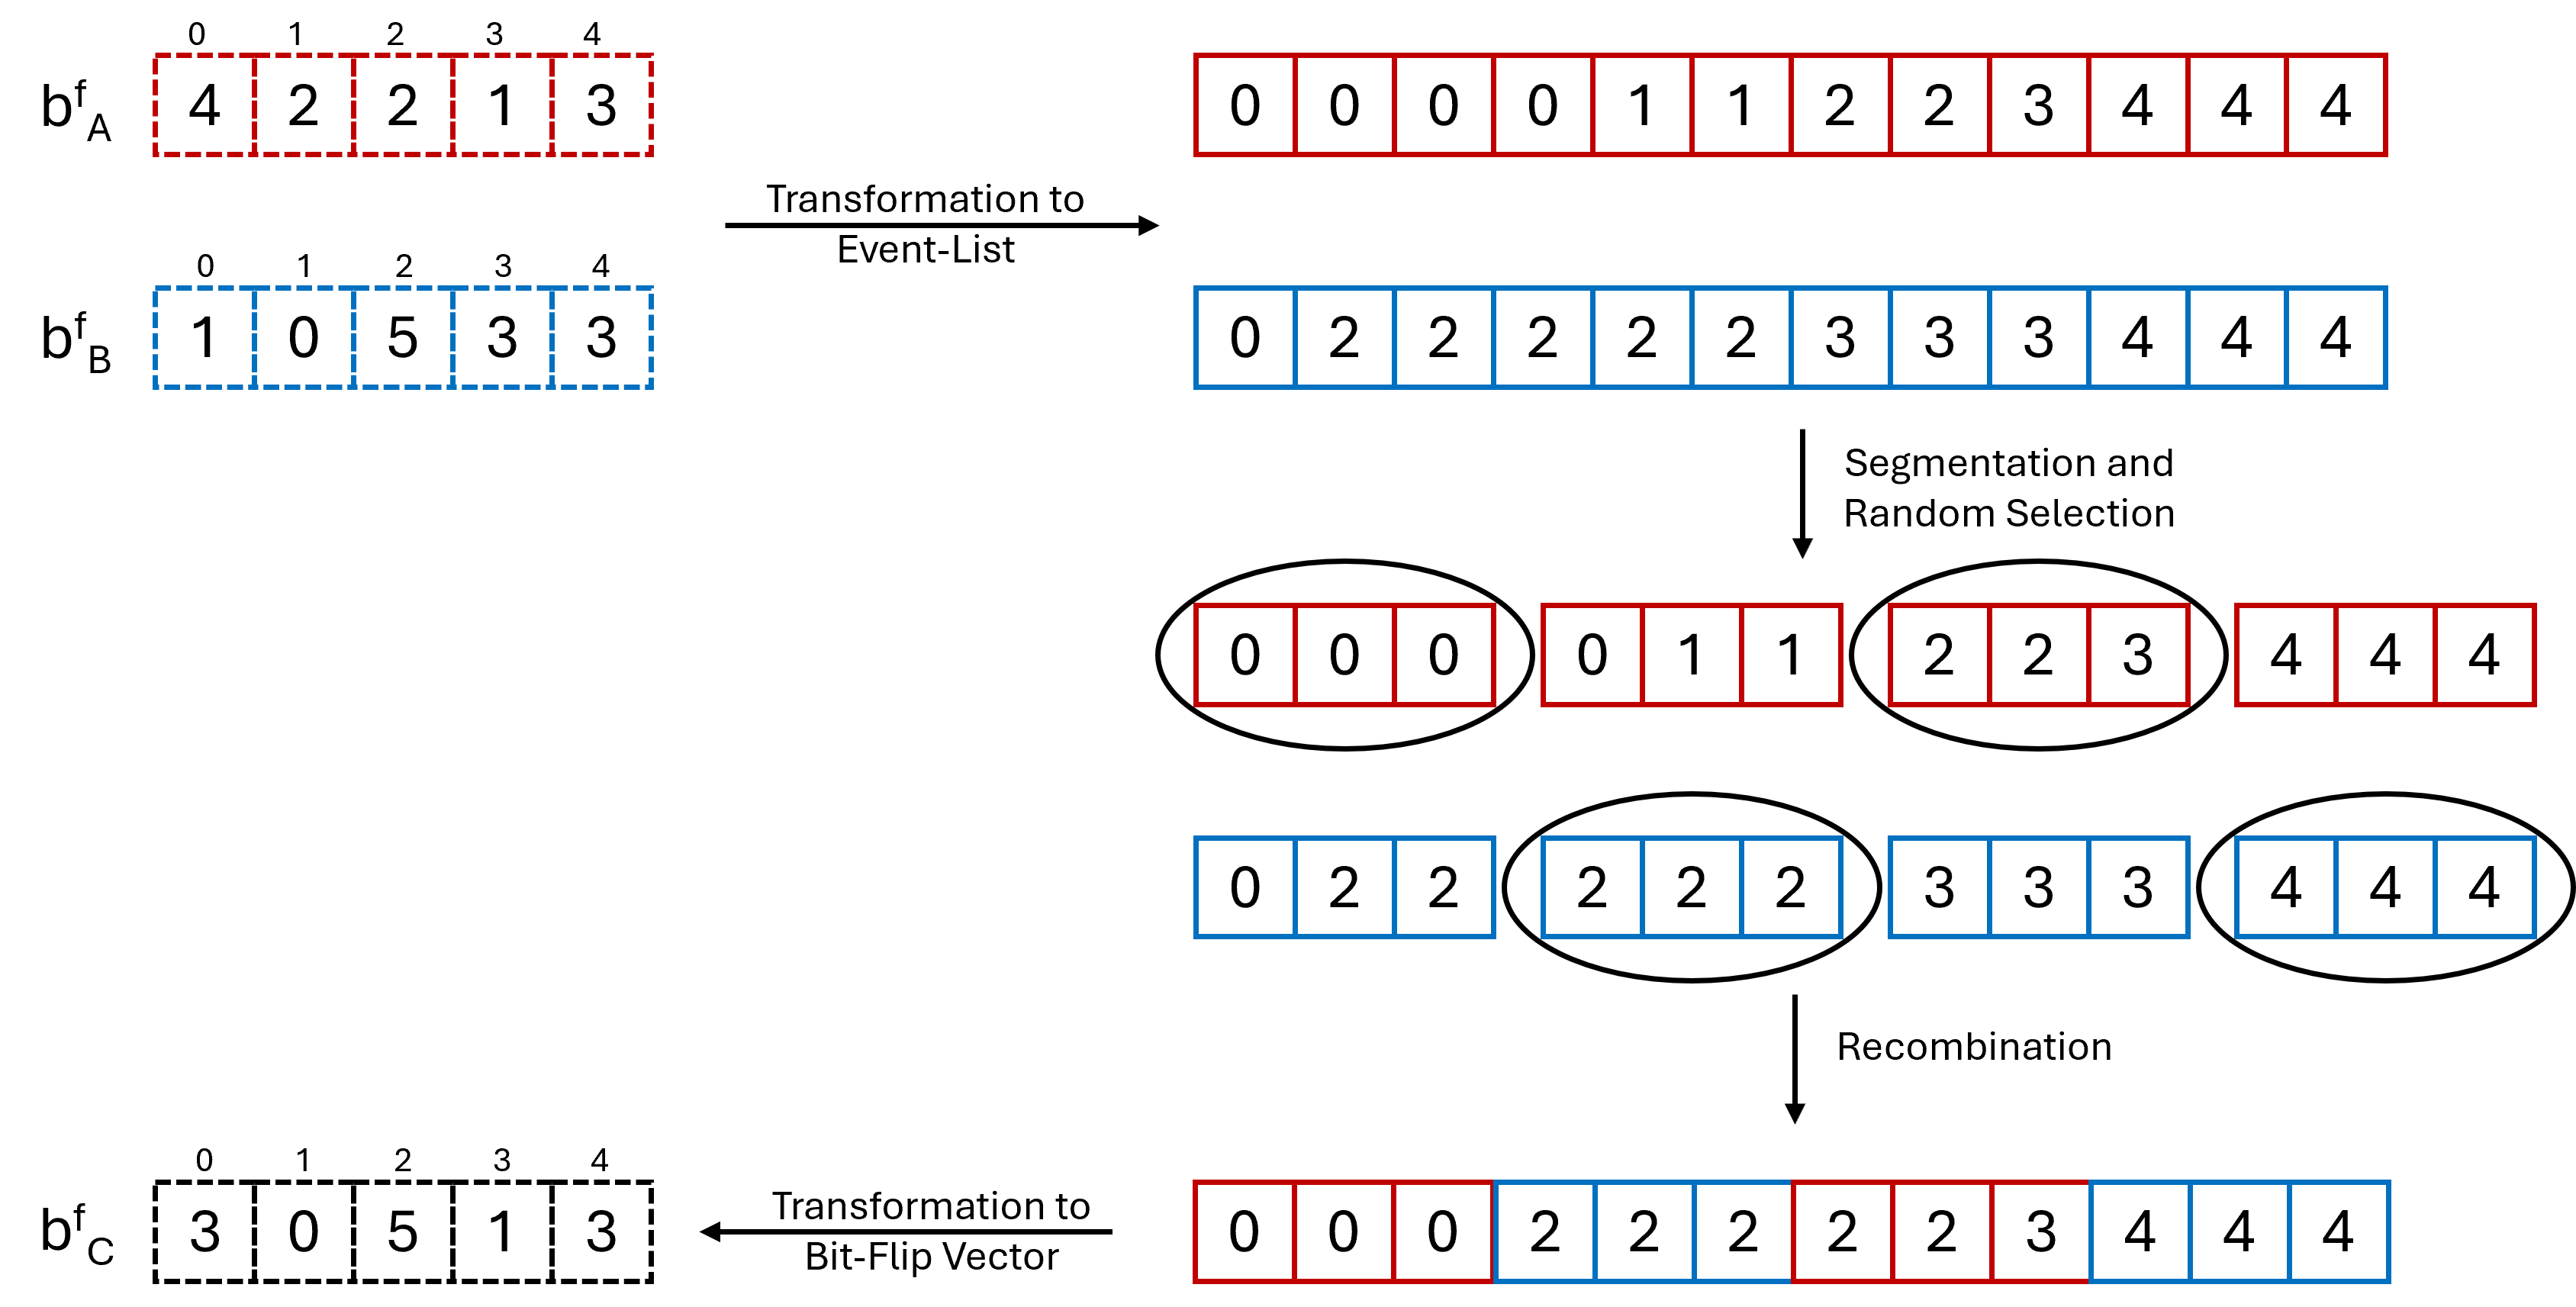
\includegraphics[width=\textwidth]{Images/ELC.png}
            \caption{Exemplary concept of the Event-List Crossover. The parent bit-flip vectors are first transformed into event lists. Crossover is then applied to segments of the event lists, and the resulting child event list is transformed back into a bit-flip vector.}
            \label{fig:event_list_crossover}
        \end{figure}
        
     A closer look at the example shows that parent $\mathbf{b}^f_A = [4, 2, 2, 1, 3]$ contains a peak of bit flips at index 0 and a minimum at index 3, while $\mathbf{b}^f_B = [1, 0, 5, 3, 3]$ has a peak at index 2 and a minimum at index 1. In the resulting child $\mathbf{b}^f_C = [3, 0, 5, 1, 3]$, the peak at index 2 inherited from $\mathbf{b}^f_B$, and the minima at indices 3 and 1 originating from $\mathbf{b}^f_A$ and $\mathbf{b}^f_B$, respectively, are preserved. Although the preservation of these structures during crossover is not guaranteed, it is more likely when complete segments rather than individual events are inherited. A peak in the bit-flip vector results in multiple consecutive occurrences of the same transition index in the event list. In this way, inheriting a segment that overlaps such a region can transfer several of these events together to the child.
     
    The degree to which characteristic extrema of both parents are preserved during crossover is therefore influenced by the segment size. Larger segments preserve longer parts of the parent event lists, while smaller segments allow more frequent switching between the two parents and therefore produce more new combinations. In GAs, this corresponds to the balance between exploration and exploitation. Early generations should provide sufficient exploration of different new candidate solutions, while later generations can increasingly exploit structures found in previous generations and refine them further. To realize this behavior in the ELC, the average segment size is adapted over the course of the optimization. The first generation uses an average segment size $\mu_{\min}$ of 0.5\% of $D$, while the final generation has an average segment size $\mu_{\max}$ of 15\% of $D$. For intermediate generations, the average segment size $\mu_g$ is interpolated geometrically as shown in Equation \ref{eq:chunk_size_mean}.
    
\begin{equation}
\mu_g =
\mu_{\min}
\left(
    \frac{\mu_{\max}}{\mu_{\min}}
\right)^{
    \frac{g-1}{G-1}
}.
\label{eq:chunk_size_mean}
\end{equation}

    Structures whose extent aligns well with a constant segment size could be more likely to be preserved than larger structures that are split across multiple segments, which may lead to segmentation artifacts. To reduce this effect, the specific size of every segment is sampled uniformly from an interval of $\pm20\%$ around the generation-dependent average segment size $\mu_g$, as shown in Equation \ref{eq:chunk_size_sampling_range}.
    
    \begin{equation}
        \mu \sim
        \mathcal{U}_{\mathbb{Z}}
        \left(
        \left\lfloor 0.8\mu_g \right\rfloor,
        \left\lfloor 1.2\mu_g \right\rfloor
        \right).
    \label{eq:chunk_size_sampling_range}
    \end{equation}
    
    Since both the segment sizes and consequently the segment boundaries in the event list are randomized, a remaining segmentation artifact could result from the first segment always starting at the first event of the list. To avoid this fixed alignment, a random offset is selected and the event list is cyclically shifted by this offset before crossover. Consequently, the segment boundaries are aligned with different positions of the event list for different crossover operations.
    
    The complete procedure is applied independently to every feature with a crossover rate of 70\%. This means that for 30\% of the features, the complete bit-flip vector $\mathbf{b}^f_A$ of parent A is copied to the child, while for the remaining 70\%, the \ac{ELC} is applied as described above.

    
    \subsection{Mutation}
    \label{sec:mutation}
    The mutation operator aims to introduce small perturbations into existing solutions to explore variations that cannot be generated by crossover alone. Without mutation, the GA could only recombine solutions already contained in the current population, but could not introduce new variations independently of the existing solutions. Mutation therefore contributes both to the local refinement of solutions and to maintaining diversity in order to reduce the risk of premature convergence \cite{hassanat_enhancing_2016}.
    
    Since directly adding or removing bit flips would violate the sum constraint, the event-list representation is also used for mutation. To preserve the total number of bit flips, a transport-based mutation is applied. Instead of adding or removing events, existing events are moved to neighboring level transitions. More specifically, mutating an event means changing its transition index in the event list by either $+1$ or $-1$. Since the number of events in the list remains unchanged, the total number of bit flips and therefore the sum constraint are preserved.

    Mutation is applied independently to every event of every feature with a probability of 20\%. If an event is selected for mutation, a direction is chosen randomly and its transition index is either increased or decreased by one. At the boundaries, cyclic wrapping is applied such that decrementing an event at the first transition maps it to the last transition and vice versa. This prevents the boundary transitions from having only one possible mutation direction, thereby reducing potential boundary artifacts.
    
    After mutation, the modified event list $\mathbf{e}^f$ is converted back into the corresponding bit-flip vector $\mathbf{b}^f$, and the resulting vectors of all features form the mutated matrix $\mathbf{B}$.



\section{Quantization}
\label{sec:quantization}
While the previous section described the optimization of where level hypervectors lie in hyperdimensional space $\mathcal{H}$ to improve class separability, the second major optimization in this work concerns how EMG values are mapped to these levels through quantization. As discussed in Section \ref{sec:optimizationOfHDCRelatedWork}, Ledwig \cite{ledwig_vdl-implementierung_2025} showed through the evaluation of different level counts that the positions of the level boundaries in the input space have a strong influence on the resulting representation and classification accuracy. 

The main goal of optimizing quantization is therefore to increase classification accuracy for a fixed number of levels or, if possible, reduce the number of levels while maintaining the accuracy of the baseline model. This directly reduces the memory required by the \ac{CCIM}, since it contains $F\times L$ hypervectors and its size therefore scales linearly with the number of levels $L$.
    \subsection{Methods}
    Quantization describes the process of mapping continuous EMG values from the input space to one of $L$ discrete levels indexed from $0$ to $L-1$. In the following, the partitioning of the input space into these discrete intervals is also referred to as binning. For every feature $f$, a set of $L-1$ thresholds $\boldsymbol{\tau}^f =[\tau^f_0,\tau^f_1,\ldots,\tau^f_{L-2}]$ is precomputed before HDC training. During encoding, the corresponding level can then be determined by comparing the feature value with the precomputed thresholds. If a value is exactly equal to a threshold, the lower adjacent level is selected. For the data-adaptive methods, the threshold vectors $\boldsymbol{\tau}^f$ are feature-specific, since the value distributions can differ between EMG electrodes and a suitable quantization for one feature is therefore not necessarily suitable for another. 

    The quantization methods evaluated in this work are grouped according to the information used to determine the thresholds. Apart from uniform binning, which is used by the baseline HDC model, two unsupervised methods, quantile binning and K-means binning, are implemented, as well as two supervised methods, decision-tree binning and ChiMerge binning.

    
        \subsubsection{Uniform Binning}
        \label{sec:UniformBinning}
        Uniform binning is the standard baseline and is used by the HDC model by default. It distributes the $L$ quantization levels uniformly over the value range, which is $[-1,1]$ for the EMG datasets used in this work, without considering the distribution of the data. The $L-1$ thresholds are placed between consecutive levels. In the implementation, Equation \ref{eq:uniform_binning_boundary} is used to precompute these thresholds with deterministic rounding and a resolution of $10^{-4}$, matching the quantization behavior of the original HDC model described in Section \ref{sec:background} and adopted from Ledwig's implementation \cite{ledwig_vdl-implementierung_2025}.

    The computation is performed using fixed-point integer arithmetic with a resolution of \(10^{-4}\). Thus, the real-valued range \([-1,1]\) is internally represented as the integer range \([-10000,10000]\). For threshold $i$, the term \(20000(i+1)-10000\), divided by $L-1$, determines the offset of the midpoint between the two corresponding uniformly spaced levels in the scaled representation. The ceiling operation followed by the subtraction of one implements the deterministic rounding behavior adopted from Ledwig’s quantization implementation \cite{ledwig_vdl-implementierung_2025}. Finally, subtracting \(10000\) shifts the result to the signed integer range corresponding to \([-1,1]\), and division by \(10000\) converts the scaled integer value back to a floating-point threshold.
    
        \begin{equation}
            \tau_i =
            \frac{
                \left\lceil
                    \frac{20000(i+1)-10000}{L-1}
                \right\rceil
                -1-10000
            }{10000},
            \qquad i=0,\ldots,L-2.
        \label{eq:uniform_binning_boundary}
        \end{equation}

        Uniform binning is the only evaluated method that is feature-independent, since its thresholds are determined only by the predefined value range and $L$, without using the training data. It therefore cannot adapt its boundaries to differences in the value distributions of individual features. It is also the most hardware-friendly of the evaluated methods, although this advantage is secondary in the proposed system because the thresholds are computed only once before training.

        
        \subsubsection{Quantile Binning}
        \label{sec:quantileBinning}

            Quantile binning is the first unsupervised method that uses the distribution of the training data and is therefore data-dependent. The main idea is to set thresholds such that the training samples are distributed approximately equally across the $L$ levels. While with uniform binning some levels may be rarely used or even unused because the corresponding value ranges contain few or no training samples, quantile binning aims to assign approximately the same number of EMG samples to every level. This results in a more balanced utilization of the available quantization levels and has the potential to improve the resulting HDC representation. Since the data distribution varies across features, separate thresholds are determined for each feature. 

            To compute the thresholds for one feature, all values of this feature in the training set are collected and sorted. The $L-1$ thresholds are then placed at the empirical quantiles according to Equation \ref{eq:quantile_binning_boundary}. $\mathbf{X}^f_{\mathrm{train}}=[x^f_0,x^f_1,\ldots,x^f_{n_{\mathrm{train}}-1}]$ denotes the sorted training values of feature $f$, with $n_{\mathrm{train}}$ as the number of training samples, and the function $\operatorname{interp}$ performs linear interpolation between neighboring sorted samples. If the quantile position lies exactly on a sample index, the corresponding sample value is used directly. Otherwise, the threshold is interpolated between the two adjacent samples.

                \begin{equation}
                \begin{aligned}
                \tau^f_{k-1}
                &=
                \operatorname{interp}
                \left(
                \mathbf{X}^f_{\mathrm{train}},
                \frac{k}{L}
                \right),
                \qquad
                k=1,\ldots,L-1,
                \\[0.5em]
                \operatorname{interp}
                \left(
                \mathbf{X}^f_{\mathrm{train}},
                q
                \right)
                &=
                (1-\alpha)x^f_{j_0} + \alpha x^f_{j_1},
                \\[0.5em]
                p
                &=
                q(n_{\mathrm{train}}-1),
                \qquad
                j_0=\lfloor p \rfloor,
                \qquad
                j_1=\lceil p \rceil,
                \\
                \alpha
                &=
                p-j_0.
                \end{aligned}
                \label{eq:quantile_binning_boundary}
                \end{equation}
           If repeated training values lead to two neighboring thresholds being equal or non-increasing, the later threshold is shifted to the next representable floating-point value. This preserves the required boundary order while changing the threshold only minimally. 
           
           Compared to uniform binning, quantile binning allocates more levels to dense regions of the feature distribution and fewer levels to sparse regions. 
           
        \subsubsection{K-Means Binning}
        \label{sec:K-meansBinning}

        K-means binning represents another data-dependent but unsupervised approach. While quantile binning distributes samples equally across bins, K-means binning instead uses the K-means clustering algorithm to search for representative centers of the EMG value distribution. The resulting thresholds are placed between neighboring cluster centers. 

        The clustering is performed separately for each feature and starts again by collecting and sorting all training values. Then $L$ cluster centers are initialized at interpolated quantile positions in the sorted training values. The algorithm repeatedly alternates between assigning each training value to its nearest center and updating each center to the mean of its assigned values. This is repeated until the center positions no longer change significantly or until the maximum number of iterations is reached. After convergence, the centers are sorted, and each threshold is computed as the midpoint between two neighboring centers. Since each value is assigned to its nearest center, these midpoints form the boundaries between neighboring clusters.

        K-means binning adapts the cluster centers to the shape of the feature distribution and can therefore represent regions with high concentrations of values more precisely. However, since the method does not use class labels, the resulting thresholds are still not necessarily aligned with class boundaries. This limitation is addressed by the following two supervised quantization methods.
        
        \subsubsection{Decision-Tree Binning}
        \label{sec:DecisiontreeBinning}
        
        Decision-tree binning is the first supervised quantization method evaluated in this work. In contrast to uniform, quantile, and K-means binning, it uses the class labels during the construction of the thresholds. The idea behind decision-tree binning is not to use the decision tree itself as a classifier, but to extract its split points as quantization boundaries. In this way, the resulting thresholds are chosen based on class separability rather than only on the distribution of feature values.

        The implementation fits one tree independently for every feature. First, all training samples are sorted by the value of the considered feature and treated as one interval. The goal is to repeatedly split the interval until $L$ subintervals are generated or no valid split remains. Therefore, the algorithm searches all currently existing intervals for the split that gives the largest reduction in sample-count-weighted Gini impurity. For each candidate split, the Gini impurities of the resulting intervals are weighted by their respective numbers of samples and compared with the weighted impurity of the interval being split.
        
        Gini impurity makes the method explicitly class-dependent. Its calculation is shown in Equation \ref{eq:gini_impurity}, where $n_c$ is the number of samples of class $c$ in an interval $S$, $|S|$ is the total number of samples in the interval, and $C$ is the number of classes.       
        A Gini impurity of 0 means that all samples in an interval belong to the same class, while increasingly mixed class distributions result in higher values of $\operatorname{Gini}(S)$. Therefore, a split is considered useful if it separates the samples into two intervals with more homogeneous class distributions. This means that the resulting thresholds are not necessarily placed in dense regions of the input distribution, but rather at positions that improve class separation. This is the main difference from quantile and K-means binning.
        
            \begin{equation}
                \operatorname{Gini}(S)
                =
                1 -
                \sum_{c=0}^{C-1}
                \left(
                    \frac{n_c}{|S|}
                \right)^2 .
            \label{eq:gini_impurity}
            \end{equation}
            
        The interval containing the best split is divided at the selected split position, and the corresponding threshold is placed halfway between the largest feature value of the left interval and the smallest feature value of the right interval. The procedure is repeated until either $L$ intervals are reached or no valid split remains. A split is only valid if both resulting intervals contain at least $\texttt{TREE\_1D\_MIN\_SAMPLES\_LEAF}=10$ samples. In addition, a candidate split is ignored if the two neighboring feature values differ by less than $\texttt{TREE\_1D\_THRESHOLD\_EPS}=10^{-12}$. This prevents thresholds from being placed between duplicate or numerically almost identical values. After tree construction, the resulting split thresholds are used directly for quantization.
        Since not every feature necessarily contains enough discriminative structure to produce \(L-1\) valid tree splits, the implementation includes a fallback mechanism. If fewer than $L-1$ thresholds are generated, the remaining thresholds are filled with quantile-based thresholds. Finally, duplicate or non-increasing thresholds are adjusted minimally to ensure strict ordering.

        Decision-tree binning therefore represents a supervised top-down approach, since it starts with one interval containing all training samples and creates finer intervals through splitting. To also evaluate the opposite family of supervised discretization methods, the next section introduces ChiMerge binning as a bottom-up approach.

        \subsubsection{ChiMerge Binning}
        \label{sec:ChiBinning}
            ChiMerge binning is the second supervised quantization method evaluated in this work. In contrast to decision-tree binning, ChiMerge follows a bottom-up approach, as it starts with a large number of small intervals and repeatedly merges neighboring intervals whose class distributions are most similar. 

            From the sorted values of each feature, the algorithm initially creates one interval for each distinct feature value. Each interval stores its value range, the number of contained samples, and a class histogram over the $C$ classes. The main idea is to repeatedly merge the two most similar adjacent intervals until only $L$ intervals remain. The similarity of two neighboring intervals is determined from their class histograms using the chi-square score.

            
            For two neighboring intervals $S_L$ and $S_R$, $n_{L,c}$ and $n_{R,c}$ denote the numbers of samples of class \(c\) in the left and right intervals, respectively. To determine whether the class distributions of the two intervals differ, these observed counts are compared with the counts that would be expected if both intervals followed the same combined class distribution. For class $c$, these expected counts are calculated as $E_{L,c}=|S_L|(n_{L,c}+n_{R,c})/(|S_L|+|S_R|)$ and $E_{R,c}=|S_R|(n_{L,c}+n_{R,c})/(|S_L|+|S_R|)$.
            The chi-square score then measures the deviation between the observed and expected counts, as shown in Equation~\ref{eq:chimerge_score}. Classes that do not occur in either interval are omitted from the calculation, since their expected counts are zero.
            
            A low chi-square score therefore indicates that the two intervals have similar class distributions and can be merged with comparatively little loss of class-separating information.
        

                \begin{equation}
                \chi^2(S_L,S_R)
                =
                \sum_{\substack{c=0\\n_{L,c}+n_{R,c}>0}}^{C-1}
                \left(
                \frac{(n_{L,c}-E_{L,c})^2}{E_{L,c}}
                +
                \frac{(n_{R,c}-E_{R,c})^2}{E_{R,c}}
                \right).
                \label{eq:chimerge_score}
                \end{equation}
            While the number of intervals is larger than $L$, the algorithm computes the chi-square score for every neighboring interval pair. The pair with the lowest chi-square score is merged, and the scores are recomputed for the updated set of intervals. After $L$ intervals are obtained, the $L-1$ thresholds are placed halfway between the intervals.
            
            Compared to decision-tree binning, ChiMerge does not search for the single best split in a larger interval. Instead, it preserves boundaries only where neighboring regions show different class distributions while removing boundaries between similar regions. This makes ChiMerge the bottom-up counterpart to the top-down decision-tree approach.\\
            
            All quantization methods produce the same output format, a threshold vector $\boldsymbol{\tau}^f$ of length $L-1$ for every feature. Therefore, the encoder and the following HDC pipeline remain unchanged, independently of the selected binning method. The quantization methods only differ in how the threshold positions are determined. Uniform binning is data-independent, quantile and K-means binning are unsupervised and use only the training values, while decision-tree and ChiMerge binning are supervised and additionally use the training labels. Their impact on HDC classification accuracy and the potential reduction of \ac{CCIM} memory through lower level counts is evaluated in Section \ref{sec:quantization_results}.\\
            

\section{FPGA Accelerator}
\label{sec:fpga_accelerator}
The previous sections described optimizations of the HDC model at the algorithmic level. 
First, redundant computations in the temporal encoding were reduced by reusing spatially encoded hypervectors. 
Then, the representation of the \ac{CCIM} was optimized with a \ac{GA}, and different quantization methods were introduced to improve the mapping from EMG feature values to discrete HDC levels. These methods improve the \ac{HDC} model itself, but they do not yet describe how the resulting pipeline can be executed efficiently on embedded hardware.

This chapter therefore describes the SystemC accelerator developed for FPGA execution of the optimized HDC pipeline. As discussed in Section \ref{sec:FPGA_background}, the binary vector operations used by HDC expose a high degree of parallelism and are well suited for FPGA implementation. The accelerator exploits this property through pipelining and different degrees of parallelism within the individual processing stages.

The accelerator does not implement the complete EMG processing workflow and is limited to the computational HDC datapath described in Section~\ref{sec:accelerator_pipeline}. Preprocessing, quantizer fitting, CCIM optimization, quantization, dataset handling, and experiment evaluation remain software tasks. 
The hardware accelerator receives already quantized EMG samples and implements spatial encoding, temporal N-gram construction, class-vector accumulation during training, and Hamming-distance computation during inference. The final class decision based on the computed distances is performed outside the accelerator.


\subsection{Hypervector Representation}
% 64-bit words
% VECTOR_WORDS = VECTOR_DIMENSION / WORD_BITS
% Why this matters for FPGA: bitwise operations over words.
In the algorithmic description, a hypervector is treated as a binary vector of dimension $D$. For the hardware implementation, the accelerator groups the vector dimensions into fixed-width words instead of representing them as individually addressed bits. Ledwig \cite{ledwig_vdl-implementierung_2025} uses a similar segmented representation in his VHDL implementation to reduce the hardware resource requirements. The word-based organization makes it possible to choose how many words are processed in parallel in each cycle. Processing more words per cycle reduces the required number of cycles, while processing fewer words allows the corresponding datapath to be reused across multiple cycles and therefore reduces hardware resource usage.


In the HDC accelerator the word width is fixed to $W = 64$ bits. The implementation requires the vector dimension $D$ to be divisible by $W$. Thus, one hypervector consists of $n_{\mathrm{words}} = \frac{D}{W}$ words and is represented as an array of $n_{\mathrm{words}}$ elements of 64 bits each. This representation is used for the CCIM, the associative memory, spatial encoding, training accumulation, and distance computation. The temporal encoding stage is an exception and internally uses a packed $D$-bit representation, since its permutation operation during N-gram construction can move bits across word boundaries. This is described in more detail in Section \ref{sec:accerator_ngram_stage}.

The word-based representation is well suited to the binary HDC operations. Binding can be performed as a bitwise XOR between corresponding words. During bundling, the bit positions within a word can be accumulated independently, while Hamming distance computation starts with a bitwise XOR followed by a population count for each word. The resulting partial Hamming distances are then added to obtain the Hamming distance over the complete hypervector.
Consequently, the representation does not change the HDC algorithm but provides a hardware-oriented organization that allows the degree of word-level parallelism to be adapted to the available hardware resources.

\subsection{Accelerator Pipeline}
\label{sec:accelerator_pipeline}

The accelerator implements the HDC processing chain as a sequence of pipeline stages. Each stage performs one part of the algorithmic pipeline and passes its result to the following stage. This separation has two main purposes. First, it allows different samples to be processed concurrently in different stages of the pipeline, thereby increasing throughput. Second, it makes the dataflow between the individual HDC operations explicit and allows the HLS tool to schedule and synthesize the operations of different stages independently.

The accelerator consists of four main processing stages for spatial encoding, temporal encoding, class-vector accumulation, and Hamming-distance computation, together with two additional stages for command handling and response generation. Each stage is implemented as a separate \texttt{SC\_CTHREAD} in SystemC. Incoming samples first pass through the command handling, spatial and temporal encoding stages. Afterwards, the temporal encoding stage routes the data according to the command type. During training, valid N-grams are forwarded to the training stage and accumulated into a class vector, while during inference, the N-grams are forwarded to the distance stage and compared with all stored class vectors. The computed distances are then passed to the response stage. The following sections describe the functional role and implementation of each stage.


Figure \ref{fig:accelerator_concept} illustrates the accelerator architecture and its main dataflow. The software controller is shown in orange, communicating with the accelerator through the AXI4-Stream wrapper in blue. The individual accelerator stages are shown in green, and the \ac{CCIM} and associative memory in purple. The arrows indicate the dataflow between the processing stages, while the separate memory-access paths show how the spatial encoder accesses the CCIM and how the associative memory is written during training and read during inference. The details of the communication interfaces, memory organization, and the individual stages are described in the following sections.



\begin{figure}[htbp]
    \centering
    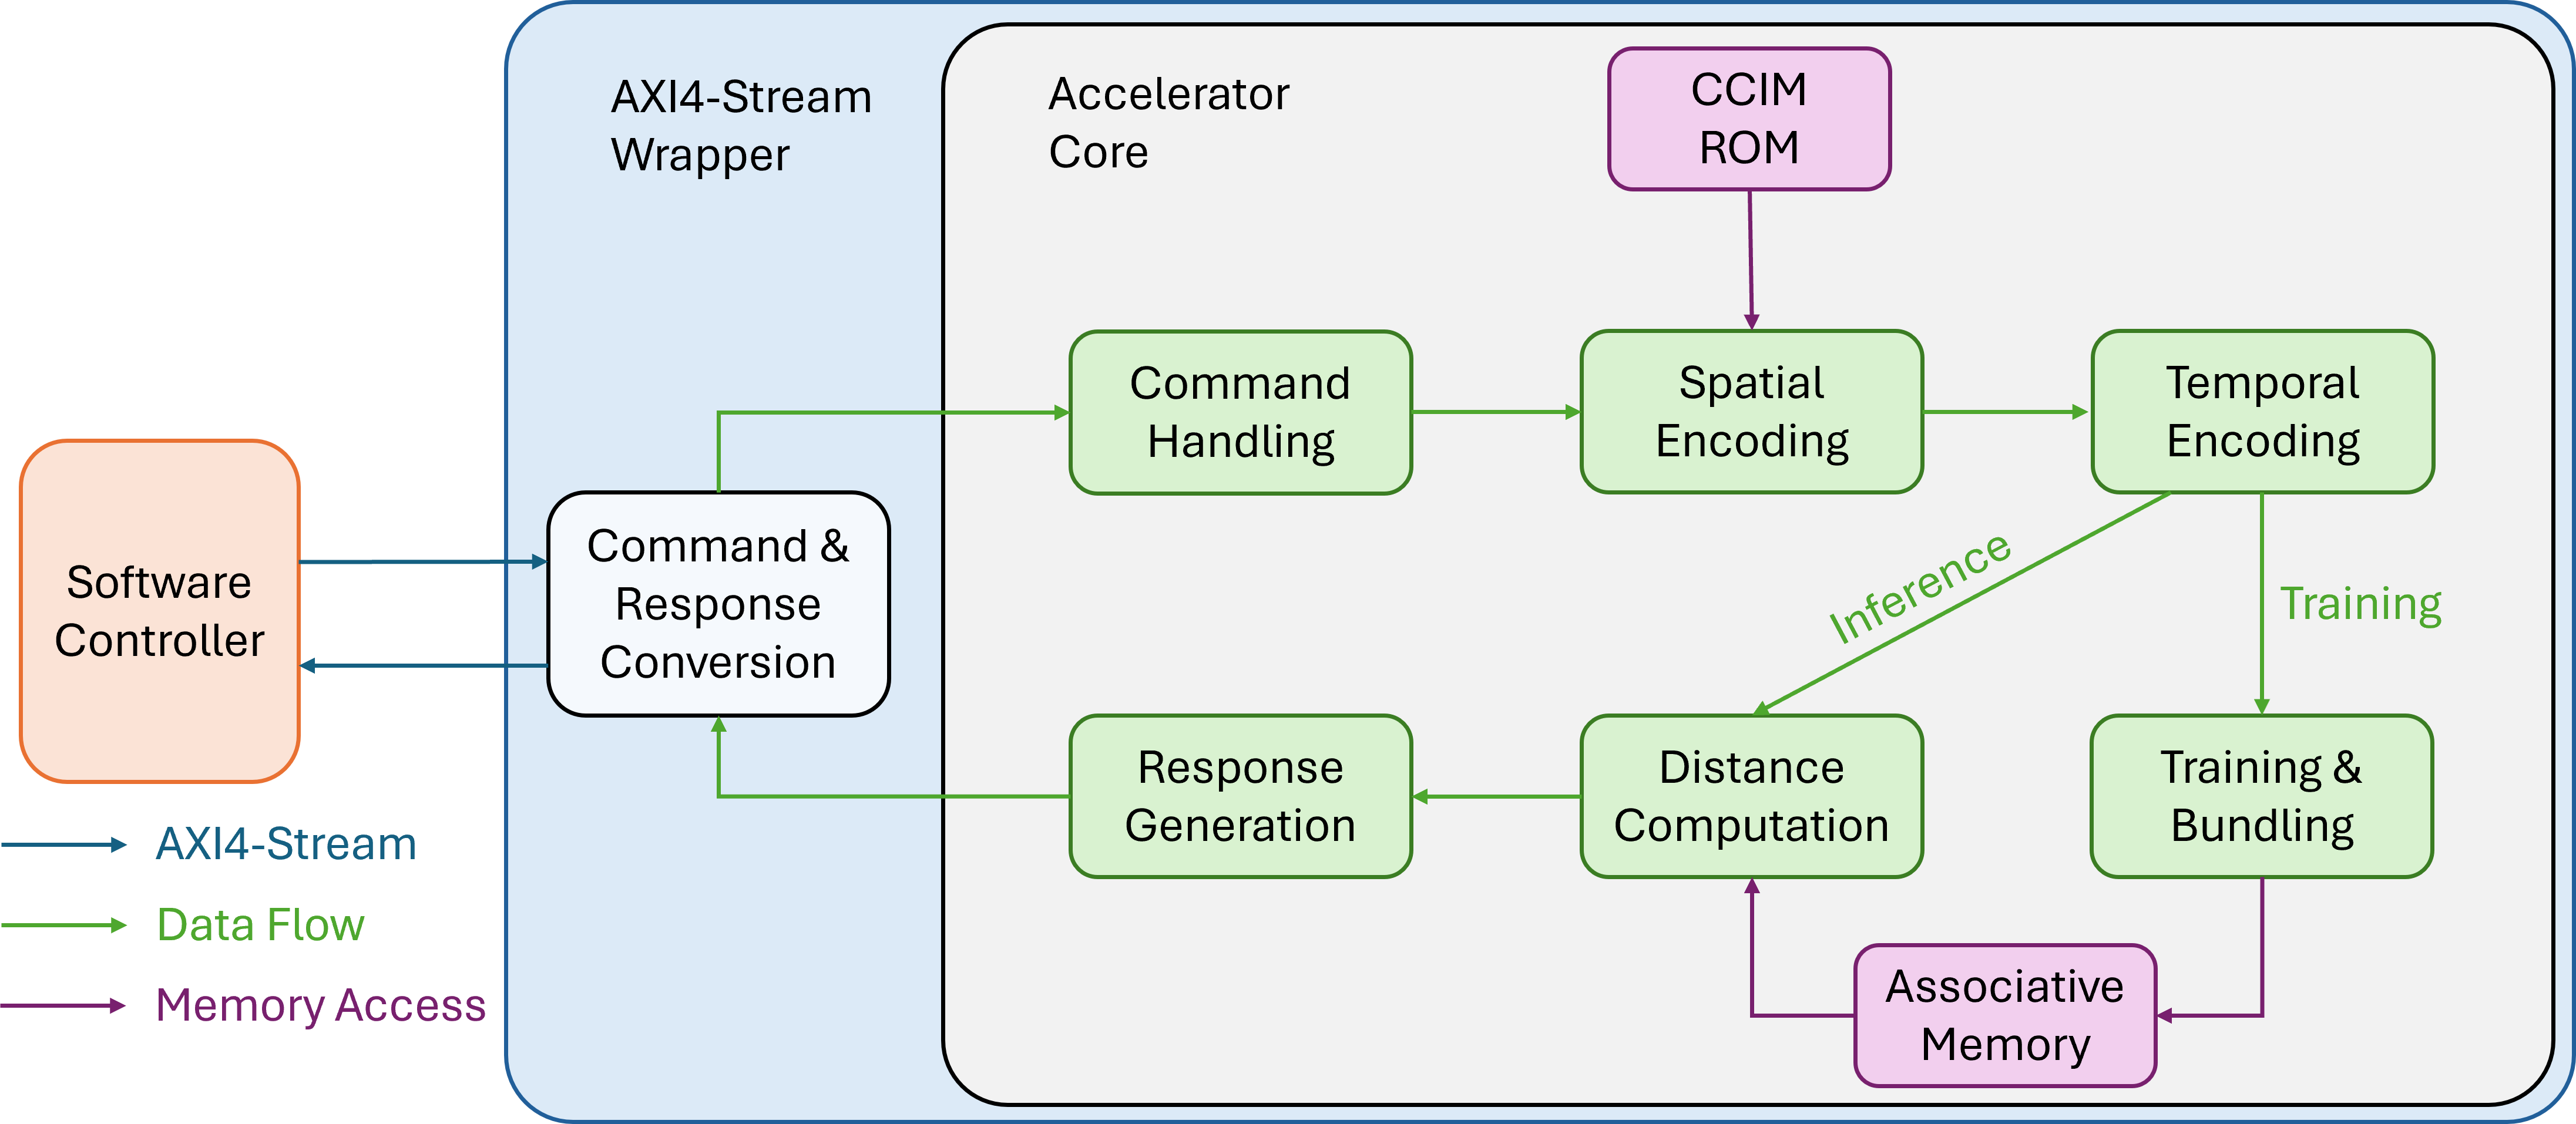
\includegraphics[width=\textwidth]
    {Images/accelerator.png}
    \caption{Overview of the HDC accelerator architecture and dataflow between the software controller in orange, AXI4-Stream wrapper in blue, accelerator pipeline in green, and internal model memories in purple.}
    \label{fig:accelerator_concept}
\end{figure}

    \subsubsection{Command Handling}
    %command stage
    The command stage forms the input stage of the accelerator core and receives commands from the software-side controller described in Section \ref{sec:controller}. It converts each command into an internal packet and forwards it to the spatial encoder. A command contains a command type, a sample consisting of 32 quantized EMG values, and, for training commands, the corresponding class ID. The command type determines how the packet is processed by the following pipeline stages. 
    
    The two types of data commands are \texttt{TrainSample} and \texttt{InferSample}. Both commands are forwarded directly into the pipeline, where the included sample is encoded. Training N-grams are then accumulated into a class vector, while inference samples are compared with the already trained \ac{AM}. The command stage does not wait for a data command to complete before accepting the next one, which allows consecutive samples to enter the accelerator while previous samples are still processed by later pipeline stages. 
    
    Control commands, in contrast, mark boundaries in the data stream and therefore require synchronization with the affected pipeline stages. They are propagated through the pipeline without encoding a sample, and the command stage waits for a completion signal before accepting further input. Three control commands are used. 

    \texttt{ResetTraining} clears both the temporal N-gram state and the current training accumulation state before a new training sequence. This prevents buffered hypervectors from the previous temporal context or unfinished bundling scores from influencing the next training sequence.

    \texttt{InvalidTrainingStep} marks a class boundary or the end of a training sequence. It clears the temporal context and, if valid N-grams have been accumulated, finalizes the current class vector by thresholding the bundling scores and writing the resulting hypervector to the associative memory.

    Finally, \texttt{ResetInference} clears only the temporal N-gram state before a new inference sequence. Since it does not modify the training state or associative memory, its completion only has to be confirmed by the temporal encoding stage.

    Through this distinction between non-blocking data commands and synchronized control commands, the command stage allows samples to flow continuously through the pipeline while ensuring that temporal and training state cannot propagate across sequence or class boundaries.
    
    \subsubsection{Spatial Encoding}
    
    The spatial encoding stage transforms one quantized EMG sample into one binary hypervector. For data commands, the incoming packet contains one quantized level index for each of the $F=32$ EMG features. These indices are used to retrieve the corresponding feature-specific level hypervectors from the \ac{CCIM}, which are then bundled into one spatial hypervector. Control commands do not contain samples to be encoded and are forwarded to the temporal encoding stage without further processing.

   The bundling operation is performed on the word-based representation described in the previous section. For each word position, the corresponding 64-bit word is retrieved from the selected CCIM hypervector of all 32 features. The implementation processes all features in parallel. For every bit position, a signed score is accumulated across the 32 feature hypervectors, with +1 for a one and -1 for a zero. The resulting output bit is set to one if the final score is greater than or equal to zero, implementing the majority operation described in Section \ref{sec:implementation_improvements}. All 64 bit positions within a word are processed in parallel.

    In addition to this feature- and bit-level parallelism, the number of hypervector words processed in one cycle can be varied. Processing more words in parallel reduces the number of cycles required for spatial encoding, but also requires additional CCIM read bandwidth and replicated bundling logic. Processing fewer words allows the same datapath to be reused over multiple cycles and reduces the corresponding hardware requirements. The memory organization that enables the required parallel CCIM accesses is described in Section~\ref{sec:accelerator_memory}.\\

    After all hypervector words have been processed, the resulting spatial hypervector is forwarded to the temporal encoding stage.
    
    \subsubsection{Temporal Encoding}
    \label{sec:accerator_ngram_stage}

    The temporal encoding stage receives the spatial hypervectors and combines consecutive samples into N-gram hypervectors. This corresponds to the temporal encoding described in Section \ref{sec:Encoding} and adds information about the recent sequence of EMG samples to the spatial representation.

    The stage stores the most recent spatial hypervectors in a ring buffer of size $N$. When a new data sample arrives, its encoded hypervector is written into the buffer and the write position is advanced. As long as fewer than $N$ valid spatial hypervectors are available, for example at the beginning of a sequence or after a control command that resets the temporal context, no valid N-gram can be generated. In this case, the stage forwards a packet with the validity flag set to false. 
    Once the buffer is filled, every newly arriving sample enables the generation of a new N-gram.

    In contrast to the word-based processing of the other stages, the temporal encoder internally represents each hypervector as one continuous $D$-bit value. This is particularly useful for permutation. While binding can be performed independently for every word, a one-bit cyclic permutation always moves bits across the boundaries between neighboring 64-bit words. A word-based implementation would therefore require explicit handling of these boundary bits for every permutation. With the continuous representation, the permutation can instead be applied directly to the complete hypervector by cyclically shifting all $D$ bits by one position. The subsequent binding operation is performed as a bitwise XOR over the complete $D$-bit vector.

    This implementation exploits full bit-level parallelism within each permutation and binding operation. Compared with processing the hypervector word by word, this avoids iterating over the $n_{\mathrm{words}}$ words for every permutation and binding operation and therefore reduces the number of cycles required for temporal encoding. The trade-off is a $D$-bit-wide permutation and XOR datapath, which requires more parallel logic and can increase routing complexity and timing pressure.\\

    Control commands reset the temporal context whenever samples from different sequences must not contribute to the same N-gram. At the beginning of inference, after a training reset, and at class transitions during training, the ring-buffer write position and the number of valid buffered hypervectors are reset. The previously stored spatial hypervectors are therefore no longer considered part of the current sequence. The following samples first refill the N-gram buffer and are forwarded as invalid N-grams until $N$ valid samples are available again.

    \subsubsection{Training and Bundling}

    The training stage receives the N-gram packets from the temporal encoding stage and constructs the class hypervectors during training. Only valid training N-grams are accumulated, while invalid N-grams are simply ignored.

    For every class, the training N-gram hypervectors are bundled by accumulating a signed score for each hypervector dimension. A bit value of one contributes +1 to the corresponding accumulator, while a zero contributes -1. Once all N-grams of a class have been processed, the accumulated scores are thresholded according to the bundling rule described in Section \ref{sec:implementation_improvements} to generate the final binary class vector, which is then stored in the \ac{AM}.

    The accumulation uses the previously described 64-bit word representation. Within each word, the 64 bit positions are updated independently and therefore in parallel.

    As in the encoder, the number of words processed in one cycle can be varied. Processing more words in parallel reduces the number of steps required to add an N-gram to the accumulator and to finalize a class vector, but requires more parallel logic and memory accesses. Processing fewer words reuses the same hardware across several word groups and consequently reduces the required resources.

    
    Class boundaries are indicated by the control commands described previously. When the current training sequence is finalized, the accumulated scores are converted into the corresponding class hypervector and written to the associative memory. The accumulation state is then cleared before samples of the next class are processed. This prevents training information from different classes from being combined.

    \subsubsection{Distance Computation}
    
    The distance computation stage is used during inference. It receives valid query hypervectors from the temporal encoding stage and compares them with the class vectors stored in the \ac{AM}. 
    For every valid inference N-gram, one Hamming distance is computed for each of the $C=5$ classes. Since these comparisons are independent, the five class distances are computed in parallel.

    For each class, the computation follows the word-based hypervector layout. The query-hypervector word and the corresponding word of the class vector stored in the \ac{AM} are XORed, producing a 64-bit difference word. The population count of this word is implemented using a fixed sequence of parallel reduction steps. Neighboring bits are first combined into partial counts, which are then successively reduced until the number of differing bits within the complete 64-bit word is obtained. Thus, the 64 individual bit differences are reduced to one partial Hamming distance for the word without checking the bits sequentially.
    
    The individual hypervector words can be compared independently, making the degree of word-level parallelism a hardware design parameter. With increasing word-level parallelism, several or all words can be compared in the same processing step. Their partial distances are then combined using a balanced reduction tree, which reduces the adder depth compared with a linear accumulation over all words. Increasing this parallelism reduces latency but also increases the amount of XOR and population-count logic, associative-memory read bandwidth, and reduction hardware.

    The distance stage does not select the final class itself. Instead, it computes the distances to all class vectors and forwards the resulting array of distances to the response stage. 
    
    \subsubsection{Response Generation}
        The response generation stage forms the output side of the accelerator pipeline. It receives the distance packet from the distance computation stage and converts it into the external response format. The response contains a validity flag and one Hamming distance value for each class. The validity flag indicates whether the corresponding inference sample produced a complete N-gram and therefore a valid set of class distances. 
        
        In the implementation, this information is packed into one response packet at the accelerator-core interface. The first bit stores the validity flag, followed by the distance values for all $C=5$ classes. This packed response is then written to the response channel. Its conversion to the AXI4-Stream interface is described separately in Section \ref{sec:Axi}.
        
        Thus, the accelerator exposes the complete distance information to the surrounding system instead of only returning a class index. 
        The final class decision is performed outside the accelerator by selecting the class with the minimum Hamming distance.

\subsection{Software Controller}
\label{sec:controller}

The accelerator does not run on its own, but is driven by a software controller. It is a software-side SystemC component and not part of the synthesized accelerator datapath. The controller defines how the accelerator is used during training and inference by generating the command stream sent to the accelerator and interpreting the returned responses. For an embedded implementation, the same control functionality can be executed on a small processor, such as a RISC-V core, connected to the accelerator through the AXI4-Stream interface described in Section \ref{sec:Axi}.

Before training, the controller sends a \texttt{ResetTraining} control command to initialize the accelerator state. It then quantizes the training samples and streams them to the accelerator using \texttt{TrainSample} commands. Whenever the class changes or the training sequence ends, the controller sends an \texttt{InvalidTrainingStep} command. This resets the temporal context and triggers the finalization and storage of the currently accumulated class vector.

During inference, the controller first sends a \texttt{ResetInference} command to reset the context of the temporal encoding stage. It then streams the quantized test samples using \texttt{InferSample} commands. For each inference sample, the accelerator returns a response containing one Hamming distance per class and a validity flag.
For valid responses, the controller selects the class with the smallest distance. In the evaluation environment, the resulting prediction is additionally compared with the reference label to determine the classification accuracy.\\

Thus, the controller performs command sequencing and coordinates training and inference, while the accelerator implements the computational HDC datapath. Dataset handling, quantization, \ac{CCIM} optimization, and experiment evaluation remain outside the synthesized hardware block, while spatial encoding, temporal encoding, training accumulation, and distance computation are performed by the accelerator.




\subsection{Inter-Stage Communication}

Inside the accelerator, the pipeline stages communicate through explicit point-to-point channels. The implementation uses \texttt{cynw\_p2p\_direct} channels between the individual \texttt{SC\_CTHREAD}s. Each channel connects one producer stage with one consumer stage and transports a fixed packet type. 
This creates a local dataflow between the processing stages without requiring central control of the internal transfers.

The command stage sends \texttt{EncoderChannelPacket}s to the spatial encoder through the channel \texttt{m\_encoder\_in}. These packets contain the command type, class identifier, quantized sample values, and a field for the encoded hypervector. For data commands, the spatial encoder fills this hypervector field with the encoded sample hypervector and forwards the packet to the temporal encoding stage through the channel \texttt{m\_encoder\_out}.

The temporal encoding stage then generates an \texttt{NGramChannelPacket}, containing the command type, class identifier, an N-gram hypervector, and a validity flag. Depending on the command type, this packet is forwarded either to the training stage through \texttt{m\_bundler\_in} or to the distance stage through \texttt{m\_distance\_in}. During inference, the resulting class distances are finally transferred to the response stage in a \texttt{DistanceChannelPacket} through \texttt{m\_distance\_done}.

The point-to-point channels also provide synchronization between the stages. A stage receives data using \texttt{get()} and forwards it using \texttt{put()}. Both operations are blocking, so a producer cannot overwrite data that has not yet been consumed and a consumer waits until new data is available. This naturally introduces backpressure into the pipeline. If a downstream stage cannot accept another packet, the preceding stages wait automatically until the dataflow can continue, without requiring additional central control logic.

Control commands require additional synchronization because they define stream boundaries. Therefore, the accelerator contains two separate completion channels. 
The channel \texttt{m\_ngram\_control\_done} is used for commands that only require completion of the temporal encoding stage, such as \texttt{ResetInference}. It connects the temporal encoding stage to the command stage and signals that the temporal context has been reset. The channel \texttt{m\_train\_control\_done} is used for the training-related control commands \texttt{ResetTraining} and \texttt{InvalidTrainingStep}. It signals that the required training-stage operation, such as resetting the accumulation state or finalizing the current class vector, has been completed. The command stage forwards the control command into the pipeline and then waits for the corresponding completion signal before accepting the next command, ensuring that no following sample crosses the respective stream boundary.

\subsection{AXI4-Stream Wrapper}
\label{sec:Axi}
The accelerator core exposes packed point-to-point channel interfaces for commands and responses. To connect these interfaces to a processor-based system, a 32-bit AXI4-Stream wrapper is added around the generated RTL. The wrapper therefore forms the external communication interface of the accelerator, while the internal command and response stages continue to use the packed Stratus point-to-point interfaces.

On the input side, the controller transmits a command as a sequence of 32-bit AXI beats. The wrapper collects these beats until the complete packed command is available and then forwards it to the command stage through the accelerator command interface. The fixed command width is determined by the widths of the command-type and class-identifier fields, the number of features, and the number of bits required to represent a quantization level. All command types use the same fixed-width format, even if parts of the payload are unused for control commands.

In the opposite direction, the response stage writes the packed response to the accelerator response interface. The wrapper divides this response into 32-bit AXI beats and transmits them to the controller. The response width depends on the number of classes and the number of bits required for each Hamming distance. Consequently, the number of required AXI beats in either direction is given by the corresponding packed interface width divided by the 32-bit AXI data width and rounded up to the next integer.

Data transfer follows the AXI4-Stream handshake using \texttt{TVALID} and \texttt{TREADY}, while \texttt{TLAST} marks the final beat of each command or response packet. The wrapper therefore bridges the processor-facing AXI4-Stream interface and the accelerator-specific packed command and response interfaces without modifying the internal HDC datapath.




\subsection{Memory Organization}
\label{sec:accelerator_memory}

The accelerator uses several internal storage structures corresponding to the HDC data structures. The main memories are the CCIM, the AM, the temporal N-gram buffer, and the bundling-score accumulator used during training. Especially for parallel processing, the memory organization must provide the required data without introducing a bottleneck that would limit the parallel datapath.\\

%CCIM
The largest model memory is the CCIM, which stores one binary level hypervector for every feature and quantization level. The CCIM is generated outside the accelerator before synthesis and not modified during training or inference. It is therefore implemented as read-only memory (ROM). To support feature-parallel spatial encoding, the CCIM is banked by feature, allowing the selected level hypervector of each of the 32 features to be accessed independently. The required additional organization depends on the degree of word-level parallelism. If several hypervector words are processed in parallel, the CCIM can additionally be banked by word to provide the required simultaneous reads. In the fully word-parallel case, each feature-word pair therefore forms an independent ROM bank containing the corresponding words of all quantization levels. This organization matches the parallelism of the spatial encoder without requiring all accesses to pass through one shared memory.

%AM
The AM stores the trained class hypervectors and is written during training and read during inference. It is organized by class and hypervector word according to the 64-bit representation. During inference, the class hypervectors are independent and their corresponding words can be accessed in parallel to support the class- and word-parallel distance computation.

%N-gram buffer
The temporal encoding stage contains a local N-gram buffer that stores the most recent spatial hypervectors. In contrast to the CCIM and AM, the buffered hypervectors are stored as continuous $D$-bit values rather than as arrays of 64-bit words. This corresponds to the packed representation used by the temporal encoder and allows permutation and binding to operate directly on the complete hypervector without explicit handling of word boundaries.
%Bundling-score accumulator
Lastly, the training stage owns an additional storage structure for class-vector accumulation. Since training first accumulates one signed score for every hypervector dimension before generating the final binary class vector, these scores must support independent updates of the individual bit positions. The bundling-score accumulator is therefore transposed by bit position. Instead of using a conventional \texttt{score[word][bit]} array, the implementation provides 64 separate bit-position banks, named \texttt{m\_bundling\_score\_0} through \texttt{m\_bundling\_score\_63}, each indexed by the hypervector word. This layout allows all 64 scores belonging to a word to be updated independently and in parallel.

\subsection{Synthesis}

The first synthesis step of the hardware implementation is the \ac{HLS} of the SystemC accelerator to an RTL description. Only the accelerator itself is part of the HLS boundary. The software controller including dataset handling, CCIM optimization, quantization, and evaluation logic is not synthesized. These components remain on the software side and are used to drive and verify the accelerator during simulation.

To make the accelerator suitable for HLS, all hardware structures have to use statically defined sizes. Array dimensions are derived from compile-time constants such as the vector dimension $D$, number of classes $C$, number of features $F$, number of quantization levels $L$, and N-gram size $N$. The external command and response interfaces are represented as packed fixed-width data types, so that only synthesizable hardware data structures cross the accelerator boundary.

The SystemC accelerator is synthesized using Cadence Stratus HLS 22.01.003. 
The HLS input consists of the six \texttt{SC\_CTHREAD}s described in the previous sections and their explicit point-to-point communication channels. Stratus schedules the operations of these processes and generates the corresponding Verilog RTL. The AXI4-Stream wrapper described in Section \ref{sec:Axi} is subsequently added around the generated accelerator core.

The resulting RTL design is verified using Vivado XSim. The RTL simulation applies the same command sequences as the SystemC simulation and compares the accelerator responses with the expected results of the reference model.
FPGA synthesis, placement, and routing are then performed using Vivado 2023.2. The FPGA targets and degrees of parallelism used for the evaluated accelerator variants are introduced together with their implementation results in Chapter~\ref{Analyse}.

The target clock period is set to 10 ns, corresponding to an accelerator clock frequency of 100 MHz, and is used as the timing constraint throughout the HLS and FPGA implementation flow. Successful implementation requires correct behavior in RTL simulation, timing closure on the target FPGA, and resource utilization within the available device capacity.\\

After optimizing the internal HDC representation and implementing the resulting model as an FPGA accelerator, the following chapter evaluates both the algorithmic optimizations and the resulting hardware implementations.